%======================================================================
\NEWMOD
%======================================================================

\section{\sDevel}

%----------------------------------------------------------------------

\logo{\hfill\hyperlink{outline<1>}{\icon}}

\begin{frame}[fragile,label=s-devel] 
\modframetitle{\sDevel}
\small
\begin{center}
\begin{minipage}{3.25in}
\begin{enumerate}
\item \hyperlink{ss-devel-coding<1>}   {\BUTTON {\ssDevelCoding}}
\item \hyperlink{ss-devel-parameter<1>}   {\BUTTON {\ssDevelParameter}}
\item \hyperlink{ss-devel-method<1>}   {\BUTTON {\ssDevelMethod}}
\item \hyperlink{ss-devel-fields<1>}   {\BUTTON {\ssDevelFields}}
\item \hyperlink{ss-devel-particles<1>}   {\BUTTON {\ssDevelParticles}}
\item \hyperlink{ss-devel-initial<1>}   {\BUTTON {\ssDevelInitial}}
\item \hyperlink{ss-devel-boundary<1>}   {\BUTTON {\ssDevelBoundary}}
\item \hyperlink{ss-devel-refine<1>}   {\BUTTON {\ssDevelRefine}}
\item \hyperlink{ss-devel-test<1>}   {\BUTTON {\ssDevelTest}}
\item \hyperlink{ss-devel-summary<1>} {\BUTTON {\ssDevelSummary}}
\end{enumerate}
\end{minipage}
\end{center}
\end{frame}

\logo{\hfill\hyperlink{s-devel<1>}{\icon}}

%======================================================================
\NEWSEC
%======================================================================

\subsection{\ssDevelCoding}

\begin{frame}[fragile,label=ss-devel-coding] 
\secframetitle{\ssDevelCoding}
\framesubtitle{Naming things}
%\footnotesize

\begin{itemize}

\item {\bluebf{Naming classes}}
%
\begin{tabbing}
xxxxxxxxxxxxxxxxxxxxxx\=xxxxxxxxxx\=\kill
\> \greenit{methods} \' \ \redcode{Enzo}\redcode{Method}\redit{Name} \\
\> \greenit{initial conditions} \'  \ \redcode{Enzo}\redcode{Initial}\redit{Name} \\
\> \greenit{boundary conditions} \'  \ \redcode{Enzo}\redcode{Boundary}\redit{Name}
\end{tabbing}
%
\item {\normalsize\bluebf{Naming files}}
%
\begin{tabbing}
xxxxxxxxxxxxxxxxxxxxxx\=xxxxxxxxxx\=\kill
\> \greenit{methods} \' \ \redcode{enzo\_Enzo}\redcode{Method}\redit{Name}\redcode{.[hc]pp} \\
\> \greenit{initial conditions} \'  \ \redcode{enzo\_Enzo}\redcode{Initial}\redit{Name}\redcode{.[hc]pp} \\
\> \greenit{boundary conditions} \'  \ \redcode{enzo\_Enzo}\redcode{Boundary}\redit{Name}\redcode{.[hc]pp}
\end{tabbing}
\end{itemize}

\end{frame}

%----------------------------------------------------------------------    

\begin{frame}[fragile] 
\secframetitle{\ssDevelCoding}
\framesubtitle{Naming things}
%
\begin{itemize}
%
\item {\normalsize\bluebf{Naming class methods}}
\begin{tabbing}
xxxxxxxxxxxxxxxxxxxxxx\=xxxxxxxxxxxxxxxxxx\=\kill
\> \greenit{public methods} \' \ \bluecode{thing\_1}\code{()} \\
\> \greenit{private methods} \' \ \bluecode{thing\_2}\redcode{\_}\code{()} \\
\> \greenit{entry methods} \' \ \redcode{p\_}\bluecode{blah}\code{()} \\
\> \greenit{reduction entry methods} \' \ \redcode{r\_}\bluecode{reduce}\code{()}
\end{tabbing}
%
\item {\normalsize\bluebf{Naming variables}}
\begin{tabbing}
xxxxxxxxxxxxxxxxxxxxxx\=xxxxxxxxxxxxxxxxxx\=\kill
\> \greenit{Array dimensions} \'  \   \bluecode{mx},\bluecode{my},\bluecode{mz} \\
\> \greenit{Active region size} \' \ \bluecode{nx},\bluecode{ny},\bluecode{nz} \\
\> \greenit{Ghost zone depth} \' \ \bluecode{gx},\bluecode{gy},\bluecode{gz} \\
\> \greenit{Loop variables} \'   \ \bluecode{ix},\bluecode{iy},\bluecode{iz} 
\end{tabbing}

\end{itemize}

\end{frame}

%----------------------------------------------------------------------    

\begin{frame}[fragile,label=field-access] 
\secframetitle{\ssDevelCoding}
\framesubtitle{Accessing field data}
\bluebf{Accessing field data is relatively easy}
\scriptsize
\newcommand{\gc}[1]{\greencode{#1}}
\newcommand{\bc}[1]{\bluecode{#1}}
\newcommand{\rc}[1]{\redcode{#1}}
\newcommand{\oc}[1]{\orangecode{#1}}
\newcommand{\mc}[1]{\magentacode{#1}}

\begin{semiverbatim}
     \gc{Field} \oc{field} = block->data()->field();

     id = field.field_id(\redcode{"density"});

     field.dimensions(id, &mx, &my, &mz);
     field.size          (&nx, &ny, &nz);
     field.ghost_depth(id &gx, &gy, &gz);

     \gc{double} * \oc{d} = (\gc{double} *) field.values(id);

     \mc{for} (\gc{int} \oc{iz}=gz; iz<gz+nz; iz++) \{
        \mc{for} (\gc{int} \oc{iy}=gy; iy<gy+ny; iy++) \{
           \mc{for} (\gc{int} \oc{ix}=gx; ix<gx+nx; ix++) \{
              \gc{int} \oc{i} = ix + mx*(iy + my*iz);
              d[i] = tiny ;
           \}
        \}
     \}
\end{semiverbatim}
\end{frame}
 % What are some coding guidelines for Enzo-P developers?
%======================================================================
\NEWSEC
%======================================================================

\subsection{\ssDevelParameter}

\begin{frame}[fragile,label=ss-devel-parameter] 
\secframetitle{\ssDevelParameter}

\begin{enumerate}
\item \bluetext{Add parameter declaration to }[\redcode{Enzo}]\redcode{Config}
\begin{tabbing}
xxxxxxxxxxxxxxxxxx\=xxxxxxxxxxxxxx\=\kill
\greentext{Cello parameter}: \> \greencode{src/Cello/parameters\_Config.hpp} \\
\greentext{Enzo parameter}: \> \greencode{src/Enzo/enzo\_EnzoConfig.hpp}
\end{tabbing}
\item \bluetext{Read parameter value in }[\redcode{Enzo}]\redcode{Config}
\begin{tabbing}
xxxxxxxxxxxxxxxxxx\=xxxxxxxxxxxxxx\=\kill
\greentext{Cello parameter}: \> \greencode{src/Cello/parameters\_Config.cpp} \\
\greentext{Enzo parameter}: \> \greencode{src/Enzo/enzo\_EnzoConfig.cpp}
\end{tabbing}
\item \bluetext{Add \charm\ pack/unpack call to} [\redcode{Enzo}]\redcode{Config}\code{::}\redcode{pup()}
\item \bluetext{Update documentation}
\begin{tabbing}
xxxxxxxxxxxxxxxxxx\=xxxxxxxxxxxxxx\=\kill
\greencode{cello-doc/source/parameters-list.rst}
\end{tabbing}
\item \bluetext{Access parameter via} [\bluecode{Enzo}]\bluecode{Config}
\end{enumerate}

\end{frame}

%----------------------------------------------------------------------

\begin{frame}[fragile]
\secframetitle{\ssDevelParameter}
\footnotesize
\bluebf{\normalsize 1.~Add parameter declaration to} \greentext{enzo\_EnzoConfig.hpp}
\begin{itemize}
\item \bluetext{Name parameter according to owning class, e.g.~for} \redcode{MethodGravityMg}
\begin{semiverbatim}
  \code{int}     \redtext{method_gravity_mg_iter_max;}
\end{semiverbatim}
\end{itemize}
\ \\
\bluebf{\normalsize 2.~Read parameter value in} \greencode{enzo\_EnzoConfig.cpp}
\begin{semiverbatim}
  \redtext{method_gravity_mg_iter_max} = \redtext{p}->\bluetext{value_integer}
    (\orangetext{"Method:gravity_mg:iter_max"},\orangetext{10});
\end{semiverbatim}
\ \\
\bluebf{\normalsize 3.~Add \charm\ pack/unpack call to} \greencode{enzo\_EnzoConfig.cpp}
\begin{semiverbatim}
void \bluetext{EnzoConfig}::\bluetext{pup} (\greentext{PUP::er} &\redtext{p}) \{
          \vdots
  \redtext{p} | \redtext{method_gravity_cg_iter_max};
          \vdots
\}
\end{semiverbatim}


\end{frame}

%----------------------------------------------------------------------

\begin{frame}[fragile]
\secframetitle{\ssDevelParameter}

\bluebf{4.~Update documentation in enzo/-doc/source/parameters-list.rst} \\
\scriptsize
\begin{semiverbatim}
\greencode{:Parameter:}  \magentacode{:p:}\greencode{`Method`} : \magentacode{:p:}\greencode{`gravity_mg`} : \magentacode{:p:}\greencode{`iter_max`}

\greencode{:Summary:} \magentacode{:s:} \greencode{`Maximum number of multigrid cycles.`}
\greencode{:Type:}    \magentacode{:t:}\greencode{`int`}
\greencode{:Default:} \magentacode{:d:}\greencode{`10`}
\greencode{:Scope:}     Enzo

\magentacode{:e:}\greencode{`Maximum number of cycles of the multigrid solver.`}
\end{semiverbatim}
\ \\
\begin{center}
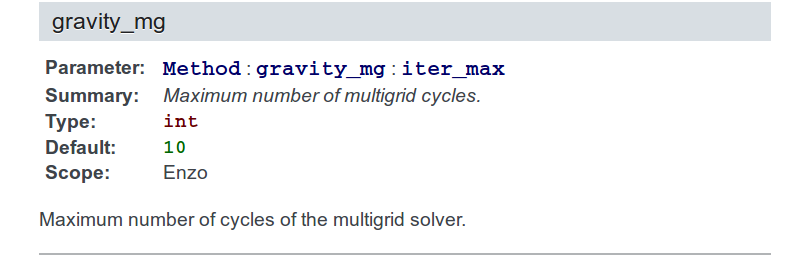
\includegraphics[width=3.5in]{mg_iter_max.png}
\end{center}
\end{frame}

%----------------------------------------------------------------------

\begin{frame}[fragile]
\secframetitle{\ssDevelParameter}
% 
 \bluebf{5.~Access parameter via \greencode{EnzoConfig} class \redcode{enzo\_config}}
\footnotesize
 \begin{semiverbatim}
\bluecode{Method} * \bluecode{EnzoProblem}::\greencode{create_method_} ()
 \{
    if (\redcode{name} == \orangecode{"ppm"}) \{
            \vdots
    \} else if (\redcode{name} == \orangecode{"gravity_mg"}) \{
       \redcode{method} = new \bluecode{EnzoMethodGravityMg0}
 	             (\redcode{field_descr}, \redcode{rank},
                    \vdots
                \redcode{enzo_config}->\redcode{method_gravity_mg_iter_max},
                    \vdots
               );
     \} \ldots
\}

\end{semiverbatim}
\end{frame}
% 
 % How do I add a new input parameter to Enzo-P?
%======================================================================
\NEWSEC
%======================================================================

\subsection{\ssDevelMethod}

\begin{frame}[fragile,label=ss-devel-method] 
\secframetitle{\ssDevelMethod}
\textbf{Suppose we wish to add a FE heat equation solver to \enzop.} \\ \ \\
\centerline{\Large \greentext{$u_t - \alpha \nabla^2 u = 0$}}
\begin{center}
\rowcolors[]{1}{blue!5}{blue!10}
  \begin{tabular}{l}
  \uncover<2->{\addclass{1.~\textbf{Create \code{EnzoMethodHeat} class}}} \\
  \uncover<3->{\addclass{2.~Include \code{enzo\_EnzoMethodHeat.hpp} file}} \\
  \uncover<4->{\addconstruct{3.~Call \code{EnzoMethodHeat} constructor}} \\
  \uncover<5->{\addparam{4.~Declare \code{EnzoMethodHeat} parameters}} \\
  \uncover<6->{\addparam{5.~Read in \code{EnzoMethodHeat} parameters}}  \\
  \uncover<7->{\addcharm{6.~Update \charm\ control file \code{enzo.ci}}} \\
  \uncover<8->{\addtest{7.~Create \code{test\_heat.in} test problem}} \\
%  \uncover<8->{\orow{Add \code{test\_heat} to the other regression tests}} \\
%  \uncover<9->{\erow{Display the \code{test\_heat} test results in \code{index.php}}} \\
  \uncover<9->{\addtest{8.~Run the test and verify test results}}
  \end{tabular}
\end{center}
\end{frame}

%----------------------------------------------------------------------

\begin{frame}[fragile] 
\secframetitle{\ssDevelMethod}
\framesubtitle{1.~Create an \code{EnzoMethodHeat} class}

\addclassbf{Create header and source code files}
      \begin{itemize}
      
         \item \textcolor{red!50!black}
             {\code{src/Enzo/enzo\_EnzoMethodHeat.hpp}}
         \item \textcolor{red!50!black}
             {\code{src/Enzo/enzo\_EnzoMethodHeat.cpp}}
      \end{itemize}
      \pause
      \bluebf{Implement virtual functions}
      \begin{itemize}
      
          \item \textcolor{blue!50!black}
              {\code{EnzoMethodHeat::EnzoMethodHeat} ()}
          \item \textcolor{blue!50!black}
              {\code{EnzoMethodHeat::compute} ()}
          \item \textcolor{blue!50!black}
              {\code{EnzoMethodHeat::timestep} ()}
          \item \textcolor{blue!50!black}
              {\code{EnzoMethodHeat::pup} ()}
      \end{itemize}
\end{frame}

\definecolor{kcol}{rgb}{0.5,0.0,0.5}
\definecolor{ccol}{rgb}{0.0,0.5,0.0}
\definecolor{mcol}{rgb}{0.8,0.0,0.0}
\definecolor{fcol}{rgb}{0.0,0.0,0.8}
\definecolor{tcol}{rgb}{0.0,0.8,0.0}
\definecolor{vcol}{rgb}{0.8,0.3,0.0}

%----------------------------------------------------------------------

\begin{frame}[fragile] 
\secframetitle{\ssDevelMethod}
\framesubtitle{1.~Create an \code{EnzoMethodHeat} class}
\addclassbf{Create the \code{src/Enzo/EnzoMethodHeat.hpp} header file}
\footnotesize
\begin{tabbing}
xxxxxxx\=xxxxxx\=\kill
\textbf<2>{\code{
\color<1,2>{kcol} class
\color<1,2>{ccol} EnzoMethodHeat
\color<1,2>{black}:\ \color<1,2>{kcol}public
\color<1,2>{ccol} Method
\color<1,2>{black}     \{ 
}}  \\
 \\[-2ex]
\code{
\color<1>{kcol} public:
\color<1>{mcol} // interface
} \\
\> \textbf<3>{\code{
\color<1,3>{fcol}  EnzoMethodHeat 
\color<1,3>{black} ( 
\color<1,3>{tcol} double 
\color<1,3>{vcol} alpha 
\color<1,3>{black} ,  
\color<1,3>{tcol} double 
\color<1,3>{vcol}  courant 
\color<1,3>{black} );
 }} \\
\> \textbf<4>{\code{
\color<1,4>{kcol} virtual 
\color<1,4>{kcol} void  
\color<1,4>{fcol} compute 
\color<1,4>{black} ( 
\color<1,4>{tcol} Block  
\color<1,4>{black} * 
\color<1,4>{vcol} block
\color<1,4>{black}) 
\color<1,4>{kcol}  throw 
\color<1,4>{black}();
}} \\
\> \textbf<4>{\code{
\color<1,4>{kcol}  virtual 
\color<1,4>{kcol}  double 
\color<1,4>{fcol}  timestep 
\color<1,4>{black}    ( 
\color<1,4>{tcol}  Block  
\color<1,4>{black}  * 
\color<1,4>{vcol}  block 
\color<1,4>{black}   )  
\color<1,4>{kcol}    throw 
\color<1,4>{black}    ();
}} \\
\> \textbf<5>{\code{
\color<1,5>{fcol}EnzoMethodHeat
\color<1,5>{black} () \{\};
}} \\
\> \textbf<5>{\code{
\color<1,5>{fcol} EnzoMethodHeat
\color<1,5>{black} (
\color<1,5>{tcol} CkMigrateMessage
\color<1,5>{black}  *
\color<1,5>{vcol} m
\color<1,5>{black} ) \{\}
}} \\
\> \textbf<5>{\code{
\color<1,5>{fcol}PUPable\_decl\color<1,5>{black}(\color<1,5>{tcol}EnzoMethodHeat\color<1,5>{black} );
}} \\
\> \textbf<5>{\code{
\color<1,5>{kcol} void
\color<1,5>{fcol} pup
\color<1,5>{black} (
\color<1,5>{tcol}PUP::er 
\color<1,5>{black}\&
\color<1,5>{vcol}p
\color<1,5>{black} )
}}
 \\
\> \textbf<5>{\code{
\color<1,5>{black} \{ 
\color<1,5>{tcol}Method\color<1,5>{black}::pup(
\color<1,5>{vcol}p
\color<1,5>{black} ); 
\color<1,5>{vcol}p
\color<1,5>{black} |
\color<1,5>{vcol} alpha\_
\color<1,5>{black} ;
\color<1,5>{vcol} p
\color<1,5>{black} |
\color<1,5>{vcol}courant\_
\color<1,5>{black} ;  \};
}} \\
\\[-2ex]
\textbf<6>{\code{
\color<1,6>{kcol} protected
\color<1,6>{black}:
\color<1,6>{mcol} // methods
}} \\
\> \textbf<6>{\code{
\color<1,6>{kcol} template 
\color<1,6>{black} $<$
\color<1,6>{kcol} class
\color<1,6>{tcol}  T
\color<1,6>{black} $>$ 
\color<1,6>{kcol} void
\color<1,6>{fcol}  compute\_ 
\color<1,6>{black} (
\color<1,6>{tcol} Block
\color<1,6>{black} * 
\color<1,6>{vcol} block
\color<1,6>{black} ,
\color<1,6>{tcol} T
\color<1,6>{black} * 
\color<1,6>{vcol} Unew
\color<1,6>{black} );
%\color<1,6>{kcol} const throw
%\color<1,6>{black} ();
}} \\
\\[-2ex]
\textbf<3>{\code{
\color<1,3>{kcol} protected
\color<1,3>{black} :
\color<1,3>{mcol}  // attributes
}} \\
\> \textbf<3>{\code{
\color<1,3>{tcol} double
\color<1,3>{vcol}  alpha\_
\color<1,3>{black} ;
}} \\
\> \textbf<3>{\code{
\color<1,3>{tcol} double
\color<1,3>{vcol}  courant\_
\color<1,3>{black} ;
}} \\
\textbf<2>{\code{
\color<1,2>{black} \};
}} \\
\end{tabbing}
\end{frame}

%-----------------------------------------------------------------------

\begin{frame}[fragile] 
\secframetitle{\ssDevelMethod}
\framesubtitle{1.~Create an \code{EnzoMethodHeat} class}
\addclassbf{Implement the \code{EnzoMethodHeat::compute()} method}
\scriptsize
\begin{semiverbatim}
\keyword{void} \type{EnzoMethodHeat}::\function{compute} ( \type{Block} * \variable{block}) throw()
\{
  \keyword{if} (\variable{block}->\function{is_leaf}()) \{

     \type{Field} \variable{field} = \variable{block}->\function{data}()->\function{field}();

     \keyword{const} \type{int} \variable{id_temp} = \variable{field}.\function{field_id} (\valuetext{"temperature"});

     \type{enzo_float} * \variable{Unew} = \variable{field}.\function{values} (\variable{id_temp});
     
     \type{field}.\function{dimensions}  (\variable{id_temp},&\variable{mx},&\variable{my},&\variable{mz});
     \type{field}.\function{ghost_depth} (\variable{id_temp},&\variable{gx},&\variable{gy},&\variable{gz});
        \vdots

  \}
  \variable{block}->\function{compute_done}();
\}
\end{semiverbatim}
\end{frame}

%----------------------------------------------------------------------

\begin{frame}[fragile] 
\secframetitle{\ssDevelMethod}
\framesubtitle{1.~Create an \code{EnzoMethodHeat} class}
\addclassbf{Implement the \code{EnzoMethodHeat::compute\_()} method}
\begin{semiverbatim}\scriptsize
        \vdots
   \keyword{for} (\type{int} \variable{iz}=\variable{gz}; \variable{iz}<\variable{mz}-\variable{gz}; \variable{iz}++) \{
      \keyword{for} (\type{int} \variable{\variable{iy}}=\variable{gy}; \variable{iy}<\variable{my}-\variable{my}; \variable{iy}++) \{
         \keyword{for} (\type{int} \variable{ix}=\variable{gx}; \variable{ix}<\variable{mx}-\variable{\variable{gx}}; \variable{ix}++) \{

            \type{int} \variable{i} = \variable{ix} + \variable{mx}*(\variable{\variable{iy}} + \variable{my}*\variable{iz});

            \type{double} \variable{Uxx} = \variable{dxi}*(\variable{U}[\variable{i}-\variable{idx}] - \valuetext{2}*\variable{U}[\variable{i}] + \variable{U}[\variable{i}+\variable{idx}]);
            \type{double} \variable{Uyy} = \variable{dyi}*(\variable{U}[\variable{i}-\variable{idy}] - \valuetext{2}*\variable{U}[\variable{i}] + \variable{U}[\variable{i}+\variable{idy}]);
            \type{double} \variable{Uzz} = \variable{dzi}*(\variable{U}[\variable{i}-\variable{idz}] - \valuetext{2}*\variable{U}[\variable{i}] + \variable{U}[\variable{i}+\variable{idz}]);

            \variable{Unew}[\variable{i}] = \variable{U}[\variable{i}] + \variable{alpha}_*\variable{dt}*(\variable{Uxx} + \variable{Uyy} + \variable{Uzz});
         \}
      \}
   \}
\}
\end{semiverbatim}
\end{frame}

%----------------------------------------------------------------------

\begin{frame}[fragile] 
\secframetitle{\ssDevelMethod}
\framesubtitle{2.~Include the \code{enzo\_EnzoMethodHeat.hpp} file}
\addclassbf{Update \code{src/Enzo/\_enzo.hpp}}
%
\begin{semiverbatim}
       \vdots
   #include "enzo_EnzoMethodPpm.hpp"
   #include "enzo_EnzoMethodPpml.hpp"
   #\keyword{include} \valuetext{"enzo_EnzoMethodHeat.hpp"}

   #include "enzo_EnzoProlong.hpp"
       \vdots
\end{semiverbatim}


\end{frame}

%----------------------------------------------------------------------

\begin{frame}[fragile] 
\secframetitle{\ssDevelMethod}
\framesubtitle{3.~Call the \code{EnzoMethodHeat} constructor}

\addconstructbf{Update \code{src/Enzo/enzo\_EnzoProblem.cpp}}
\footnotesize
\begin{semiverbatim}
   Method * EnzoProblem::create_method_ (\dots)
   \{
         \vdots
      if (type == "ppm") \{
          method = new EnzoMethodPpm;
      \} else if (type == "ppml") \{
          method = new EnzoMethodPpml;
      \} \keyword{else if} (\variable{type} == \valuetext{"heat"}) \{
          \variable{method} = \keyword{new} \type{EnzoMethodHeat}
             (\variable{enzo_config->method_heat_alpha,}
              \variable{enzo_config->method_courant});
      \} else if
         \vdots
   \}
\end{semiverbatim}

\end{frame}

%----------------------------------------------------------------------

\begin{frame}[fragile, label=ss-devel-parameters] 
\secframetitle{\ssDevelMethod}
\framesubtitle{4.~Declare any \code{EnzoMethodHeat} parameters}

\addparambf{Update \code{src/Enzo/enzo\_EnzoConfig.hpp}}
\footnotesize
\begin{semiverbatim}
   class EnzoConfig : public Config \{
        \vdots 
   public: // attributes
        \vdots
     std::string      interpolation_method;

     \comment{// EnzoMethodHeat}
     \keyword{double}           \variable{method_heat_alpha};
        \vdots 
   \};
\end{semiverbatim}

\end{frame}

%======================================================================

\begin{frame}[fragile] 
\secframetitle{\ssDevelMethod}
\framesubtitle{5.~Read in the \code{EnzoMethodHeat} parameters}

\addparambf{Update \code{src/Enzo/enzo\_EnzoConfig.cpp}}
\footnotesize
\begin{semiverbatim}
   void EnzoConfig::read(\dots)
   \{
        \vdots
      interpolation_method = p->value_string 
        ("Field:interpolation_method","SecondOrderA");

      \variable{method_heat_alpha} = \variable{p}->\function{value_float}
        (\valuetext{"Method:heat:alpha"},\valuetext{1.0});

      method_null_dt = p->value_float 
        ("Method:null:dt",std::numeric_limits<double>::max());
        \vdots
   \}
\end{semiverbatim}

\end{frame}

%======================================================================

\begin{frame}[fragile] 
\secframetitle{\ssDevelMethod}
\framesubtitle{6.~Update the \charm\ control file \code{enzo.ci}}

\addcharmbf{Update \code{src/Enzo/enzo.ci}}
\footnotesize
\begin{semiverbatim}
   module enzo \{
       \vdots
     PUPable EnzoInitialImplosion2;
     PUPable EnzoInitialSedovArray2;
     PUPable EnzoInitialSedovArray3;
     PUPable EnzoMethodPpm;
     PUPable EnzoMethodPpml;
     \type{PUPable} \variable{EnzoMethodHeat};
     PUPable EnzoProblem;
       \vdots
   \};
\end{semiverbatim}
\end{frame}


%======================================================================

\begin{frame}[fragile] 
\secframetitle{\ssDevelMethod}
\framesubtitle{7.~Create a \code{test\_heat.in} test problem}
\addtestbf{Create \code{input/test\_heat.in}}
\scriptsize
\vspace{-0.15in}
\begin{semiverbatim}
      \vdots
   \group{Method} \{
     \parameter{list} = [\valuetext{"heat"}]; 
     \subgroup{heat} \{ \parameter{alpha} = \valuetext{1.0}; \} 
     \parameter{courant} = \valuetext{0.5};
   \}
\pause
   \group{Field} \{
      \parameter{list} = [\valuetext{"temperature"}];
   \}
\pause
   \group{Adapt} \{
      \parameter{list} = [\valuetext{"slope"}];
      \subgroup{slope} \{
         \parameter{type} = \valuetext{"slope"};
         \parameter{field_list} = [\valuetext{"temperature"}];
      \}
   \}
\end{semiverbatim}

\end{frame}

%----------------------------------------------------------------------

% \begin{frame}[fragile] 
% \secframetitle{\ssDevelMethod}
% \framesubtitle{Add \code{test\_heat} to the other regression tests}
% 
% \code{test/SConscript}
% 
% \begin{center}
% \begin{minipage}{3.0in}
% \blockblue
% \begin{block}<+->{\textbf{\code{src/Enzo/enzo\_EnzoProblem.cpp}}}
% \footnotesize
% \begin{semiverbatim}
% 
% test/SConscript:# MethodHeat tests
% test/SConscript:Clean(env\_mv\_out.RunSerial ('test\_method\_heat-1.unit',bin% \_path + '/enzo-p', 
% test/SConscript:		ARGS='input/method\_heat-1.in'),
% test/SConscript:      [Glob('#/' + test\_path + '/method\_heat-1*.png'),
% test/SConscript:       Glob('#/' + test\_path + '/method\_heat-1*.h5'),
% test/SConscript:        '#/input/method\_heat-1.in.out'])
% test/SConscript:env.MakeMovie ("method\_heat-1.swf", "test\_method\_heat-1.unit", \
% test/SConscript:                ARGS= test\_path + "/method\_heat-1*.png");
% test/SConscript:Clean(env\_mv\_out.RunParallel ('test\_method\_heat-8.unit',bin\_path + '/enzo-p', 
% test/SConscript:		ARGS='input/method\_heat-8.in'),
% test/SConscript:      [Glob('#/' + test\_path + '/method\_heat-8*.png'),
% test/SConscript:      Glob('#/' + test\_path + '/method\_heat-8*.h5'),
% test/SConscript:      '#/input/method\_heat-8.in.out'])
% test/SConscript:env.MakeMovie ("method\_heat-8.swf", "test\_method\_heat-8.unit", \
% test/SConscript:                ARGS= test\_path + "/method\_heat-8-*.png");
% \end{semiverbatim}
% \end{block}
% \end{minipage}
% \end{center}
% \end{frame}

%----------------------------------------------------------------------

% \begin{frame}[fragile] 
% \secframetitle{\ssDevelMethod}
% \framesubtitle{Display the \code{test\_heat} test results in \code{index.php}}
     
% \code{test/index.php}


% \begin{center}
% \begin{minipage}{3.0in}
% \blockblue
% \begin{block}<+->{\textbf{\code{src/Enzo/enzo\_EnzoProblem.cpp}}}
% \footnotesize
% \begin{semiverbatim}
% test/index.php:test\_summary("Method-heat",
% test/index.php:	     array("method\_heat-1",
% test/index.php:		   "method\_heat-8"),
% test/index.php:test\_group("Method-heat");
% test/index.php:Method-heat tests serve to test basic functionality of the "heat" method
% test/index.php:  echo "<h3>HEAT (serial) </h3>";
% test/index.php:tests("Enzo","enzo-p","test\_method\_heat-1","HEAT 1 block");
% test/index.php:test\_table ("method\_heat-1",
% test/index.php:  echo "<h3>HEAT (parallel) </h3>";
% test/index.php:tests("Enzo","enzo-p","test\_method\_heat-8","HEAT 8 block");
% test/index.php:test\_table ("method\_heat-8",
% \end{semiverbatim}
% \end{block}
% \end{minipage}
% \end{center}
% \end{frame}

%----------------------------------------------------------------------


\begin{frame}[fragile] 
\secframetitle{\ssDevelMethod}
\framesubtitle{8.~Run the test and verify test results}
%     Call test problem in \code{test/}
\begin{center}
  \ANIMATEGRAPHICS{controls,width=3.5in}{20}{Images/HeatAmr/heat-}{000}{300}
\end{center}
\end{frame}

%----------------------------------------------------------------------

% \begin{frame}[fragile] 
% \secframetitle{\ssDevelMethod}
% \framesubtitle{8.~Run the test and verify test results}
%    \addtestbf{Lets make it unstable and see what happens! (bwahaha)}\\
%    \centerline{\code{\group{Field} \{ \parameter{courant} = \valuetext{1.1}; \} }}
% \begin{center}
%   \ANIMATEGRAPHICS{controls,width=3.5in}{5}{Images/HeatUnstable/heat-00}{000}{100}
% \end{center}
% \end{frame}

 % How do I add a new method to Enzo-P?
%======================================================================
\NEWSEC
%======================================================================

\subsection{\ssDevelFields}

\begin{frame}[fragile,label=ss-devel-fields] 
\secframetitle{\ssDevelFields}
\end{frame}

 % How write a Method using Fields?
%======================================================================
\NEWSEC
%======================================================================

\subsection{\ssDevelParticles}

\begin{frame}[fragile,label=ss-devel-particles] 
\secframetitle{\ssDevelParticles}
\end{frame}

 % How do I write a Method using Particles?
%======================================================================
\NEWSEC
%======================================================================

\subsection{\ssDevelInitial}

\begin{frame}[fragile,label=ss-devel-initial] 
\secframetitle{\ssDevelInitial}
\textbf{Suppose we wish to add an implosion test problem to \enzop.}\begin{center}
\rowcolors[]{1}{blue!5}{blue!10}
  \begin{tabular}{l}
  \uncover<2->{\addclass{1.~\textbf{Create \code{EnzoInitialImplosion2} class}}} \\
  \uncover<3->{\addclass{2.~Include \code{enzo\_EnzoInitialImplosion2.hpp} file}} \\
  \uncover<4->{\addconstruct{3.~Call \code{EnzoInitialImplosion2} constructor}} \\
  \uncover<5->{\addparam{4.~Declare any \code{EnzoInitialImplosion2} parameters}} \\
  \uncover<6->{\addparam{5.~Read in any \code{EnzoInitialImplosion2} parameters}}  \\
  \uncover<7->{\addcharm{6.~Update \charm\ control file \code{enzo.ci}}} \\
  \uncover<8->{\addtest{7.~Create \code{test\_implosion.in} test problem}} \\
  \uncover<9->{\addtest{8.~Run the test and verify test results}}
  \end{tabular}
\end{center}

\end{frame}

%----------------------------------------------------------------------

\begin{frame}[fragile] 
\secframetitle{\ssDevelInitial}
\framesubtitle{1.~Create an \code{EnzoInitialImplosion2} class}

\addclassbf{Create header and source code files}
      \begin{itemize}
      
         \item \textcolor{red!50!black}
             {\code{src/Enzo/enzo\_EnzoInitialImplosion2.hpp}}
         \item \textcolor{red!50!black}
             {\code{src/Enzo/enzo\_EnzoInitialImplosion2.cpp}}
      \end{itemize}
      \pause
      \bluebf{Implement virtual functions}
      \begin{itemize}
      
          \item \textcolor{blue!50!black}
              {\code{EnzoInitialImplosion2::EnzoInitialImplosion2} ()}
          \item \textcolor{blue!50!black}
              {\code{EnzoInitialImplosion2::enforce\_block} ()}
          \item \textcolor{blue!50!black}
              {\code{EnzoInitialImplosion2::pup} ()}
      \end{itemize}
\end{frame}

\definecolor{kcol}{rgb}{0.5,0.0,0.5}
\definecolor{ccol}{rgb}{0.0,0.5,0.0}
\definecolor{mcol}{rgb}{0.8,0.0,0.0}
\definecolor{fcol}{rgb}{0.0,0.0,0.8}
\definecolor{tcol}{rgb}{0.0,0.8,0.0}
\definecolor{vcol}{rgb}{0.8,0.3,0.0}

%----------------------------------------------------------------------

\begin{frame}[fragile] 
\secframetitle{\ssDevelInitial}
\framesubtitle{1.~Create an \code{EnzoInitialImplosion2} class}
\addclassbf{Create the \code{src/Enzo/EnzoInitialImplosion2.hpp} header file}
\footnotesize
\begin{tabbing}
xxxxxxx\=xxxxxx\=\kill
\textbf<2>{\code{
\color<1,2>{kcol} class
\color<1,2>{ccol} EnzoInitialImplosion2
\color<1,2>{black}:\ \color<1,2>{kcol}public
\color<1,2>{ccol} Initial
\color<1,2>{black}     \{ 
}}  \\
 \\[-2ex]
\code{
\color<1>{kcol} public:
\color<1>{mcol} // interface
} \\
\> \textbf<3>{\code{
\color<1,3>{fcol}  EnzoInitialImplosion2 
\color<1,3>{black} ( 
\color<1,3>{tcol}  int
\color<1,3>{black}  * 
\color<1,3>{vcol}  cycle 
\color<1,3>{black}  ,
\color<1,3>{tcol}  double  
\color<1,3>{black}  * 
\color<1,3>{vcol}  time
\color<1,3>{black} );
 }} \\
\> \textbf<4>{\code{
\color<1,4>{kcol} virtual 
\color<1,4>{kcol} void  
\color<1,4>{fcol} enforce\_block
}} \\
\> \> \textbf<4>{\code{
\color<1,4>{black}    ( 
\color<1,4>{tcol}  Block  
\color<1,4>{black}  * 
\color<1,4>{vcol}  block 
\color<1,4>{black}  ,
}} \\
\> \> \textbf<4>{\code{
\color<1,4>{tcol}  \ \ const FieldDescr
\color<1,4>{black}  * 
\color<1,4>{vcol}  field\_descr
\color<1,4>{black}  , 
}} \\
\> \> \textbf<4>{\code{
\color<1,4>{tcol}  \ \ const Hierarchy
\color<1,4>{black}  * 
\color<1,4>{vcol}  hierarchy
\color<1,4>{black}   )  
\color<1,4>{kcol}    throw 
\color<1,4>{black}    ();
}} \\
\> \textbf<5>{\code{
\color<1,5>{fcol}EnzoInitialImplosion2
\color<1,5>{black} () \{\};
}} \\
\> \textbf<5>{\code{
\color<1,5>{fcol} EnzoInitialImplosion2
\color<1,5>{black} (
\color<1,5>{tcol} CkMigrateMessage
\color<1,5>{black}  *
\color<1,5>{vcol} m
\color<1,5>{black} ) \{\}
}} \\
\> \textbf<5>{\code{
\color<1,5>{fcol}PUPable\_decl\color<1,5>{black}(\color<1,5>{tcol}EnzoInitialImplosion2\color<1,5>{black} );
}} \\
\> \textbf<5>{\code{
\color<1,5>{kcol} void
\color<1,5>{fcol} pup
\color<1,5>{black} (
\color<1,5>{tcol}PUP::er 
\color<1,5>{black}\&
\color<1,5>{vcol}p
\color<1,5>{black} )
}}
 \\
\> \textbf<5>{\code{
\color<1,5>{black} \{ 
\color<1,5>{tcol}Initial\color<1,5>{black}::pup(
\color<1,5>{vcol}p
\color<1,5>{black} ); 
\color<1,5>{black} \};
}} \\
\ \code{\}}
\end{tabbing}
\end{frame}

%-----------------------------------------------------------------------

\begin{frame}[fragile] 
\secframetitle{\ssDevelInitial}
\framesubtitle{1.~Create an \code{EnzoInitialImplosion2} class}
\addclassbf{Implement the \code{EnzoInitialImplosion2::enforce\_block()} method}
\scriptsize
\begin{semiverbatim}
\keyword{void} \type{EnzoInitialImplosion2}::\function{enforce_block} 
(
 \type{Block} * \variable{block},
 \keyword{const} \type{FieldDescr} * \variable{field_descr},
 \keyword{const} \type{Hierarchy}  * \variable{hierarchy}
 ) \keyword{throw}()
\{
   \type{Field} \variable{field} = \variable{block}->\function{data}()->\function{field}();

   \type{enzo_float} *  \variable{d} = (\type{enzo_float} *) \variable{field}.\function{values}(\valuetext{"density"});
   \type{enzo_float} * \variable{vx} = (\type{enzo_float} *) \variable{field}.\function{values}(\valuetext{"velocity_x}");
   \type{enzo_float} * \variable{vy} = (\type{enzo_float} *) \variable{field}.\function{values}(\valuetext{"velocity_y}");
   \type{enzo_float} * \variable{te} = (\type{enzo_float} *) \variable{field}.\function{values}(\valuetext{"total_energy}");
      \vdots
\end{semiverbatim}
\end{frame}

%-----------------------------------------------------------------------

\begin{frame}[fragile] 
\secframetitle{\ssDevelInitial}
\framesubtitle{1.~Create an \code{EnzoInitialImplosion2} class}
\addclassbf{Implement the \code{EnzoInitialImplosion2::enforce\_block()} method}
\scriptsize
\begin{semiverbatim}
      \vdots
  \comment{// Field attributes}
  \type{int} \variable{mx},\variable{my},\variable{gx},\variable{gy};     
  \variable{field}.\function{dimensions}  (\valuetext{0},&\variable{mx},&\variable{my});
  \variable{field}.\function{ghost_depth} (\valuetext{0},&\variable{gx},&\variable{gy});

  \comment{// Cell widths}
  \type{double} \variable{hx},\variable{hy};
  \variable{block}->\function{cell_width}(&\variable{hx},&\variable{hy});
      \vdots
\end{semiverbatim}
\end{frame}

%-----------------------------------------------------------------------

\begin{frame}[fragile] 
\secframetitle{\ssDevelInitial}
\framesubtitle{1.~Create an \code{EnzoInitialImplosion2} class}
\addclassbf{Implement the \code{EnzoInitialImplosion2::enforce\_block()} method}
\scriptsize
\begin{semiverbatim}
      \vdots
   \keyword{for} (\type{int} \variable{iy}=\variable{gy}; \variable{iy}<\variable{my}-\variable{gy}; \variable{iy}++) \{
      \type{double} \variable{y} = \variable{ym} + (\variable{iy} - \variable{gy} + \valuetext{0.5})*\variable{hy};
      \keyword{for} (\type{int} \variable{ix}=\variable{gx}; \variable{ix}<\variable{mx}-\variable{gx}; \variable{ix}++) \{
         \type{double} \variable{x} = \variable{xm} + (\variable{ix} - \variable{gx} + \valuetext{0.5})*\variable{hx};
         \type{int} \variable{i} = \variable{ix} + \variable{mx}*\variable{iy};
         \keyword{if} (\variable{x} + \variable{y} < \valuetext{0.1517}) \{
            \variable{d}[\variable{i}]  = \valuetext{0.125};
            \variable{te}[\variable{i}] = \valuetext{0.14} / ((\type{EnzoBlock}::\variable{Gamma} - \valuetext{1.0}) * \variable{d}[\variable{i}]);
         \} \keyword{else} \{
            \variable{d}[\variable{i}]  = \valuetext{1.0};
            \variable{te}[\variable{i}] = \valuetext{1.0} / ((\type{EnzoBlock}::\variable{Gamma} - \valuetext{1.0}) * \variable{d}[\variable{i}]);
         \}
         \variable{vx}[\variable{i}] = \variable{vy}[\variable{i}] = \valuetext{0.0};
      \}
   \}
\}
\end{semiverbatim}
\end{frame}

%----------------------------------------------------------------------

\begin{frame}[fragile] 
\secframetitle{\ssDevelInitial}
\framesubtitle{2.~Include the \code{enzo\_EnzoInitialImplosion2.hpp} file}

\addclassbf{Update \code{src/Enzo/\_enzo.hpp}}
%
\begin{semiverbatim}
       \vdots
   #include "enzo_EnzoInitialGrackleTest.hpp"
   #\keyword{include} \valuetext{"enzo_EnzoInitialImplosion2.hpp"}
   #include "enzo_EnzoInitialSedovArray2.hpp"
   #include "enzo_EnzoInitialSedovArray3.hpp"
   #include "enzo_EnzoInitialTurbulence.hpp"
       \vdots
\end{semiverbatim}


\end{frame}

%----------------------------------------------------------------------

\begin{frame}[fragile] 
\secframetitle{\ssDevelInitial}
\framesubtitle{3.~Call the \code{EnzoInitialImplosion2} constructor}

\addconstructbf{Update \code{src/Enzo/enzo\_EnzoProblem.cpp}}
\footnotesize
\begin{semiverbatim}
   Initial * EnzoProblem::create_initial_ (\dots)
   \{
         \vdots
       \keyword{if} (\variable{type} == \valuetext{"implosion_2d"}) \{
         \variable{initial} = \keyword{new} \type{EnzoInitialImplosion2}(\variable{cycle},\variable{time});
       \} else if (type == "sedov_array_2d") \{
         initial = new EnzoInitialSedovArray2(enzo_config);
       \} else if (type == "sedov_array_3d") \{
         initial = new EnzoInitialSedovArray3(enzo_config);
         \vdots
   \}
\end{semiverbatim}

\end{frame}

%----------------------------------------------------------------------

\begin{frame}[fragile] 
\secframetitle{\ssDevelInitial}
\framesubtitle{4--5.~Handle any parameters}
\addparambf{(No parameters: see section on \hyperlink{ss-devel-parameters}{\underline{adding parameters to \code{Method}s)}}}
\end{frame}

%======================================================================

\begin{frame}[fragile] 
\secframetitle{\ssDevelInitial}
\framesubtitle{6.~Update the \charm\ control file \code{enzo.ci}}

\addcharmbf{Update \code{src/Enzo/enzo.ci}}
\footnotesize
\begin{semiverbatim}
   module enzo \{
       \vdots
     \type{PUPable} \variable{EnzoInitialImplosion2};
     PUPable EnzoInitialSedovArray2;
     PUPable EnzoInitialSedovArray3;
     PUPable EnzoInitialTurbulence;
       \vdots
   \};
\end{semiverbatim}
\end{frame}


%======================================================================

\begin{frame}[fragile] 
\secframetitle{\ssDevelInitial}
\framesubtitle{7.~Create a \code{test\_implosion.in} test problem}
\addtestbf{Create \code{input/test\_implosion.in}}
\vspace{-0.15in}
\begin{semiverbatim}
      \vdots
   \group{Initial} \{
      \parameter{list} = [\valuetext{"implosion_2d"}]; 
   \}
      \vdots
\end{semiverbatim}

\end{frame}

%----------------------------------------------------------------------

% \begin{frame}[fragile] 
% \secframetitle{\ssDevelInitial}
% \framesubtitle{Add \code{test\_heat} to the other regression tests}
% 
% \code{test/SConscript}
% 
% \begin{center}
% \begin{minipage}{3.0in}
% \blockblue
% \begin{block}<+->{\textbf{\code{src/Enzo/enzo\_EnzoProblem.cpp}}}
% \footnotesize
% \begin{semiverbatim}
% 
% test/SConscript:# InitialImplosion tests
% test/SConscript:Clean(env\_mv\_out.RunSerial ('test\_initial\_heat-1.unit',bin% \_path + '/enzo-p', 
% test/SConscript:		ARGS='input/initial\_heat-1.in'),
% test/SConscript:      [Glob('#/' + test\_path + '/initial\_heat-1*.png'),
% test/SConscript:       Glob('#/' + test\_path + '/initial\_heat-1*.h5'),
% test/SConscript:        '#/input/initial\_heat-1.in.out'])
% test/SConscript:env.MakeMovie ("initial\_heat-1.swf", "test\_initial\_heat-1.unit", \
% test/SConscript:                ARGS= test\_path + "/initial\_heat-1*.png");
% test/SConscript:Clean(env\_mv\_out.RunParallel ('test\_initial\_heat-8.unit',bin\_path + '/enzo-p', 
% test/SConscript:		ARGS='input/initial\_heat-8.in'),
% test/SConscript:      [Glob('#/' + test\_path + '/initial\_heat-8*.png'),
% test/SConscript:      Glob('#/' + test\_path + '/initial\_heat-8*.h5'),
% test/SConscript:      '#/input/initial\_heat-8.in.out'])
% test/SConscript:env.MakeMovie ("initial\_heat-8.swf", "test\_initial\_heat-8.unit", \
% test/SConscript:                ARGS= test\_path + "/initial\_heat-8-*.png");
% \end{semiverbatim}
% \end{block}
% \end{minipage}
% \end{center}
% \end{frame}

%----------------------------------------------------------------------

% \begin{frame}[fragile] 
% \secframetitle{\ssDevelInitial}
% \framesubtitle{Display the \code{test\_heat} test results in \code{index.php}}
     
% \code{test/index.php}


% \begin{center}
% \begin{minipage}{3.0in}
% \blockblue
% \begin{block}<+->{\textbf{\code{src/Enzo/enzo\_EnzoProblem.cpp}}}
% \footnotesize
% \begin{semiverbatim}
% test/index.php:test\_summary("Initial-heat",
% test/index.php:	     array("initial\_heat-1",
% test/index.php:		   "initial\_heat-8"),
% test/index.php:test\_group("Initial-heat");
% test/index.php:Initial-heat tests serve to test basic functionality of the "heat" initial
% test/index.php:  echo "<h3>HEAT (serial) </h3>";
% test/index.php:tests("Enzo","enzo-p","test\_initial\_heat-1","HEAT 1 block");
% test/index.php:test\_table ("initial\_heat-1",
% test/index.php:  echo "<h3>HEAT (parallel) </h3>";
% test/index.php:tests("Enzo","enzo-p","test\_initial\_heat-8","HEAT 8 block");
% test/index.php:test\_table ("initial\_heat-8",
% \end{semiverbatim}
% \end{block}
% \end{minipage}
% \end{center}
% \end{frame}

%----------------------------------------------------------------------


\begin{frame}[fragile] 
\secframetitle{\ssDevelInitial}
\framesubtitle{8.~Run the test and verify test results}
%     Call test problem in \code{test/}
\begin{center}
  \ANIMATEGRAPHICS{controls,width=2.0in}{20}{Images/Implosion/d-0}{000}{200}
\end{center}
\end{frame}

 % How do I add initial conditions to Enzo-P?
%======================================================================
\NEWSEC
%======================================================================

\subsection{\ssDevelBoundary}

\begin{frame}[fragile,label=ss-devel-boundary] 
\secframetitle{\ssDevelBoundary}
\textbf{Suppose we wish to add outflow boundary conditions to \enzop.}
\begin{center}
\rowcolors[]{1}{blue!5}{blue!10}
  \begin{tabular}{l}
  \uncover<2->{\addclass{1.~\textbf{Create \code{EnzoBoundaryOutflow} class}}} \\
  \uncover<3->{\addclass{2.~Include \code{enzo\_EnzoBoundaryOutflow.hpp} file}} \\
  \uncover<4->{\addconstruct{3.~Call \code{EnzoBoundaryOutflow} constructor}} \\
  \uncover<5->{\addparam{4.~Declare any \code{EnzoBoundaryOutflow} parameters}} \\
  \uncover<6->{\addparam{5.~Read in any \code{EnzoBoundaryOutflow} parameters}}  \\
  \uncover<7->{\addcharm{6.~Update \charm\ control file \code{enzo.ci}}} \\
  \uncover<8->{\addtest{7.~Create \code{test\_outflow.in} test problem}} \\
  \uncover<9->{\addtest{8.~Run the test and verify test results}}
  \end{tabular}
\end{center}
\  \\
(Currently implemented in \code{EnzoBoundary})

\end{frame}

%----------------------------------------------------------------------

\begin{frame}[fragile] 
\secframetitle{\ssDevelBoundary}
\framesubtitle{\addclass{1.~Create an \code{EnzoBoundaryOutflow} class}}

\addclassbf{Create header and source code files}
      \begin{itemize}
      
         \item \textcolor{red!50!black}
             {\code{src/Enzo/enzo\_EnzoBoundaryOutflow.hpp}}
         \item \textcolor{red!50!black}
             {\code{src/Enzo/enzo\_EnzoBoundaryOutflow.cpp}}
      \end{itemize}
      \pause
      \bluebf{Implement virtual functions}
      \begin{itemize}
      
          \item \addclass{\code{EnzoBoundaryOutflow::EnzoBoundaryOutflow} ()}
          \item \addclass{\code{EnzoBoundaryOutflow::enforce} ()}
          \item \addclass{\code{EnzoBoundaryOutflow::pup} ()}
      \end{itemize}
\end{frame}

\definecolor{kcol}{rgb}{0.5,0.0,0.5}
\definecolor{ccol}{rgb}{0.0,0.5,0.0}
\definecolor{mcol}{rgb}{0.8,0.0,0.0}
\definecolor{fcol}{rgb}{0.0,0.0,0.8}
\definecolor{tcol}{rgb}{0.0,0.8,0.0}
\definecolor{vcol}{rgb}{0.8,0.3,0.0}

%----------------------------------------------------------------------

\begin{frame}[fragile] 
\secframetitle{\ssDevelBoundary}
\framesubtitle{\addclass{1.~Create an \code{EnzoBoundaryOutflow} class}}
\addclassbf{Create the \code{src/Enzo/EnzoBoundaryOutflow.hpp} header file}
\footnotesize
\begin{tabbing}
xxxxxxx\=xxxxxx\=\kill
\textbf<2>{\code{
\color<1,2>{kcol} class
\color<1,2>{ccol} EnzoBoundaryOutflow
\color<1,2>{black}:\ \color<1,2>{kcol}public
\color<1,2>{ccol} Boundary
\color<1,2>{black}     \{ 
}}  \\
 \\[-2ex]
\code{
\color<1>{kcol} public:
\color<1>{mcol} // interface
} \\
\> \textbf<3>{\code{
\color<1,3>{fcol}  EnzoBoundaryOutflow 
}} \\
\> \> \textbf<4>{\code{
\color<1,3>{black}   ( 
\color<1,3>{tcol}  axis\_enum
\color<1,3>{vcol}  axis 
\color<1,3>{black}  ,
\color<1,3>{tcol}  face\_enum
\color<1,3>{vcol}  face 
\color<1,3>{black}  ,
\color<1,3>{tcol}  Mask
\color<1,3>{black}  * 
\color<1,3>{vcol}  mask
\color<1,3>{black} );
 }} \\
\> \textbf<4>{\code{
\color<1,4>{kcol} virtual 
\color<1,4>{kcol} void  
\color<1,4>{fcol} enforce
}} \\
\> \> \textbf<4>{\code{
\color<1,4>{black}    ( 
\color<1,4>{tcol}  Block  
\color<1,4>{black}  * 
\color<1,4>{vcol}  block 
\color<1,4>{black}  ,
 }} \\
\> \> \textbf<3>{\code{
\color<1,4>{tcol} \ \  face\_enum
\color<1,4>{vcol}  face 
\color<1,4>{black}  ,
\color<1,4>{tcol}  axis\_enum
\color<1,4>{vcol}  axis 
\color<1,4>{black}   )  
\color<1,4>{kcol}    throw 
\color<1,4>{black}    ();
}} \\
\> \textbf<5>{\code{
\color<1,5>{fcol}EnzoBoundaryOutflow
\color<1,5>{black} () \{\};
}} \\
\> \textbf<5>{\code{
\color<1,5>{fcol} EnzoBoundaryOutflow
\color<1,5>{black} (
\color<1,5>{tcol} CkMigrateMessage
\color<1,5>{black}  *
\color<1,5>{vcol} m
\color<1,5>{black} ) \{\}
}} \\
\> \textbf<5>{\code{
\color<1,5>{fcol}PUPable\_decl\color<1,5>{black}(\color<1,5>{tcol}EnzoBoundaryOutflow\color<1,5>{black} );
}} \\
\> \textbf<5>{\code{
\color<1,5>{kcol} void
\color<1,5>{fcol} pup
\color<1,5>{black} (
\color<1,5>{tcol}PUP::er 
\color<1,5>{black}\&
\color<1,5>{vcol}p
\color<1,5>{black} )
}}
 \\
\> \textbf<5>{\code{
\color<1,5>{black} \{ 
\color<1,5>{tcol}Boundary::pup
\color<1,5>{black} (
\color<1,5>{vcol}p
\color<1,5>{black} ); 
\color<1,5>{black} \};
}} \\
\ \code{\}}
\end{tabbing}
\end{frame}

%-----------------------------------------------------------------------

\begin{frame}[fragile] 
\secframetitle{\ssDevelBoundary}
\framesubtitle{\addclass{1.~Create an \code{EnzoBoundaryOutflow} class}}
\addclassbf{Implement the \code{EnzoBoundaryOutflow} constructor}
\begin{semiverbatim}
   \type{EnzoBoundary}::\function{EnzoBoundary} 
   ( \type{axis_enum} \variable{axis},
     \type{face_enum} \variable{face}, 
     \type{Mask} * \variable{mask} ) \keyword{throw}()
     : \type{Boundary}(\variable{axis},\variable{face},\variable{mask})
   \{  \}
\end{semiverbatim}


\end{frame}

%-----------------------------------------------------------------------

\begin{frame}[fragile] 
\secframetitle{\ssDevelBoundary}
\framesubtitle{\addclass{1.~Create an \code{EnzoBoundaryOutflow} class}}
\addclassbf{Implement the \code{EnzoBoundaryOutflow::enforce()} method (1/4)}
\scriptsize
\begin{semiverbatim}
\keyword{void} \type{EnzoBoundaryOutflow}::\function{enforce} 
( \type{Block} * \variable{block}, \type{face_enum} \variable{face}, \type{axis_enum} \variable{axis} ) \keyword{throw}()
\{
  \comment{// Skip if not applicable}
  \keyword{if} ( ! \function{applies_}(\variable{axis}, \variable{face})) \keyword{return};

  \keyword{if} (\variable{face} == \variable{face_all}) \{
    \function{enforce}(\variable{block}, \variable{face_lower},\variable{axis});
    \function{enforce}(\variable{block}, \variable{face_upper},\variable{axis});
  \} \keyword{else if} (\variable{axis} == \variable{axis_all}) \{
    \function{enforce}(\variable{block}, \variable{face,axis_x});
    \function{enforce}(\variable{block}, \variable{face,axis_y});
    \function{enforce}(\variable{block}, \variable{face,axis_z});
  \} \keyword{else} \{
      \vdots
\end{semiverbatim}
\end{frame}

%-----------------------------------------------------------------------

\begin{frame}[fragile] 
\secframetitle{\ssDevelBoundary}
\framesubtitle{\addclass{1.~Create an \code{EnzoBoundaryOutflow} class}}
\addclassbf{Implement the \code{EnzoBoundaryOutflow::enforce()} method (2/4)}
\scriptsize
\vspace{-0.15in}
\begin{semiverbatim}
      \vdots
   \type{Data} * \variable{data} = \variable{block}->\function{data}();
   \type{Field} \variable{field} = \variable{data}->\function{field}();

   \comment{// Field attributes}
   \type{int} \variable{nx},\variable{ny},\variable{nz};
   \variable{field}.\function{size}(&\variable{nx},&\variable{ny},&\variable{nz});

   \comment{// Cell centers if needed for Mask}
   \type{double} *\variable{x}=\valuetext{0}, *\variable{y}=\valuetext{0}, *\variable{z}=\valuetext{0};
   \keyword{if} (\variable{mask_}) \{
      \variable{x} = \type{new} \type{double} [\variable{nx}];
      \variable{y} = \type{new} \type{double} [\variable{ny}];
      \variable{z} = \type{new} \type{double} [\variable{nz}];
      \variable{data}->\function{field_cells}(\variable{x},\variable{y},\variable{z});
   \}
      \vdots
\end{semiverbatim}
\end{frame}

%-----------------------------------------------------------------------

\begin{frame}[fragile] 
\secframetitle{\ssDevelBoundary}
\framesubtitle{\addclass{1.~Create an \code{EnzoBoundaryOutflow} class}}
\addclassbf{Implement the \code{EnzoBoundaryOutflow::enforce()} method (3/4)}
\vspace{-0.15in}
\scriptsize
\begin{semiverbatim}
      \vdots
   \comment{// Coordinates of Block edges}
   \type{double} \variable{xm},\variable{ym},\variable{zm};
   \type{double} \variable{xp},\variable{yp},\variable{zp};
   \variable{data} -> \function{lower}(&\variable{xm},&\variable{ym},&\variable{zm});
   \variable{data} -> \function{upper}(&\variable{xp},&\variable{yp},&\variable{zp});

   \type{double} t = \variable{block}->\function{time}();

   \comment{// @@@ BUG: loops through all fields!}
   \keyword{for} (\keyword{int} \variable{index} = 0; \variable{index} < \variable{field}.\function{field_count}(); \variable{index}++) \{

      \variable{field}.\function{dimensions}  (\variable{index},&\variable{mx},&\variable{my},&\variable{mz});
      \variable{field}.\function{ghost_depth} (\variable{index},&\variable{gx},&\variable{gy},&\variable{gz});

      \type{enzo_float} * \variable{array} = (\type{enzo_float} *) \variable{field}.\function{values}(\variable{index});
      \vdots

\end{semiverbatim}
\end{frame}

%-----------------------------------------------------------------------

\begin{frame}[fragile] 
\secframetitle{\ssDevelBoundary}
\framesubtitle{\addclass{1.~Create an \code{EnzoBoundaryOutflow} class}}
\addclassbf{Implement the \code{EnzoBoundaryOutflow::enforce()} method (4/4)}
\vspace{-0.15in}
\scriptsize
\begin{semiverbatim}
      \vdots
      \keyword{if} (\variable{face} == \variable{face_lower} && \variable{axis} == \variable{axis_x}) \{
         \keyword{if} (\variable{nx} > \valuetext{1}) \{
            \keyword{for} (\variable{iz}=\variable{0}; \variable{iz}<\variable{mz}; \variable{iz}++) \{
               \keyword{for} (\variable{iy}=\variable{0}; \variable{iy}<\variable{my}; \variable{iy}++) \{
                  \keyword{for} (\variable{ix}=\variable{0}; \variable{ix}<\variable{gx}; \variable{ix}++) \{
                     \keyword{int} \variable{i_internal} = \variable{gx}      + \variable{mx}*(\variable{iy} + \variable{my}*\variable{iz});
                     \keyword{int} \variable{i_external} = \variable{gx}-\variable{ix}-\valuetext{1} + \variable{mx}*(\variable{iy} + \variable{my}*\variable{iz});
                     \keyword{if} (! \variable{mask_} || \variable{mask_}->\function{evaluate}(\variable{t},\variable{xm},\variable{y}[\variable{iy}],\variable{z}[\variable{iz}]))
                        \variable{array}[\variable{i_external}] = \variable{array}[\variable{i_internal}];
              \}
           \}
        \}
     \}
      \vdots
\end{semiverbatim}
\end{frame}

%----------------------------------------------------------------------

\begin{frame}[fragile] 
\secframetitle{\ssDevelBoundary}
\framesubtitle{\addclass{2.~Include the \code{enzo\_EnzoBoundaryOutflow.hpp} file}}

\addclassbf{Update \code{src/Enzo/\_enzo.hpp}}
%
\begin{semiverbatim}
       \vdots
   #\keyword{include} \valuetext{"enzo_EnzoBoundaryOutflow.hpp"}
       \vdots
\end{semiverbatim}


\end{frame}

%----------------------------------------------------------------------

\begin{frame}[fragile] 
\secframetitle{\ssDevelBoundary}
\framesubtitle{\addconstruct{3.~Call the \code{EnzoBoundaryOutflow} constructor}}

\addconstructbf{Update \code{src/Enzo/enzo\_EnzoProblem.cpp}}
\footnotesize
\begin{semiverbatim}
   Boundary * EnzoProblem::create_boundary_ (\dots)
   \{
         \vdots
   if (       type == "reflecting") \{ 
      boundary = new EnzoBoundary 
         (axis,face,mask,boundary_type_reflecting);
   \} \keyword{else if} (\variable{type} == \valuetext{"outflow"}) \{
      \variable{boundary} = \keyword{new} \type{EnzoBoundaryOutflow} (\variable{axis},\variable{face},\variable{mask});
   \} else \{
      boundary = Problem::create_boundary_
         (type,index,config,parameters);
   \}
         \vdots
   \}
\end{semiverbatim}

\end{frame}

%----------------------------------------------------------------------

\begin{frame}[fragile] 
\secframetitle{\ssDevelBoundary}
\framesubtitle{4--5.~Handle any parameters}
\addparambf{(No parameters: see section on \hyperlink{ss-devel-parameters}{\underline{adding parameters to \code{Method}s)}}}
\end{frame}

%======================================================================

\begin{frame}[fragile] 
\secframetitle{\ssDevelBoundary}
\framesubtitle{6.~Update the \charm\ control file \code{enzo.ci}}

\addcharmbf{Update \code{src/Enzo/enzo.ci}}
\footnotesize
\begin{semiverbatim}
   module enzo \{
       \vdots
      \type{PUPable} \type{EnzoBoundary};
       \vdots
   \};
\end{semiverbatim}
\end{frame}


%======================================================================

\begin{frame}[fragile] 
\secframetitle{\ssDevelBoundary}
\framesubtitle{7-8.~Create a \code{test\_outflow.in} test problem}
\addtestbf{Create \code{input/test\_outflow.in}}
\vspace{-0.15in}
\begin{semiverbatim}
      \vdots
   \group{Boundary} \{
      \parameter{type} = [\valuetext{"outflow"}]; 
   \}
      \vdots
\end{semiverbatim}

\end{frame}

%----------------------------------------------------------------------

% \begin{frame}[fragile] 
% \secframetitle{\ssDevelBoundary}
% \framesubtitle{Add \code{test\_heat} to the other regression tests}
% 
% \code{test/SConscript}
% 
% \begin{center}
% \begin{minipage}{3.0in}
% \blockblue
% \begin{block}<+->{\textbf{\code{src/Enzo/enzo\_EnzoProblem.cpp}}}
% \footnotesize
% \begin{semiverbatim}
% 
% test/SConscript:# BoundaryOutflow tests
% test/SConscript:Clean(env\_mv\_out.RunSerial ('test\_boundary\_heat-1.unit',bin% \_path + '/enzo-p', 
% test/SConscript:		ARGS='input/boundary\_heat-1.in'),
% test/SConscript:      [Glob('#/' + test\_path + '/boundary\_heat-1*.png'),
% test/SConscript:       Glob('#/' + test\_path + '/boundary\_heat-1*.h5'),
% test/SConscript:        '#/input/boundary\_heat-1.in.out'])
% test/SConscript:env.MakeMovie ("boundary\_heat-1.swf", "test\_boundary\_heat-1.unit", \
% test/SConscript:                ARGS= test\_path + "/boundary\_heat-1*.png");
% test/SConscript:Clean(env\_mv\_out.RunParallel ('test\_boundary\_heat-8.unit',bin\_path + '/enzo-p', 
% test/SConscript:		ARGS='input/boundary\_heat-8.in'),
% test/SConscript:      [Glob('#/' + test\_path + '/boundary\_heat-8*.png'),
% test/SConscript:      Glob('#/' + test\_path + '/boundary\_heat-8*.h5'),
% test/SConscript:      '#/input/boundary\_heat-8.in.out'])
% test/SConscript:env.MakeMovie ("boundary\_heat-8.swf", "test\_boundary\_heat-8.unit", \
% test/SConscript:                ARGS= test\_path + "/boundary\_heat-8-*.png");
% \end{semiverbatim}
% \end{block}
% \end{minipage}
% \end{center}
% \end{frame}

%----------------------------------------------------------------------

% \begin{frame}[fragile] 
% \secframetitle{\ssDevelBoundary}
% \framesubtitle{Display the \code{test\_heat} test results in \code{index.php}}
     
% \code{test/index.php}


% \begin{center}
% \begin{minipage}{3.0in}
% \blockblue
% \begin{block}<+->{\textbf{\code{src/Enzo/enzo\_EnzoProblem.cpp}}}
% \footnotesize
% \begin{semiverbatim}
% test/index.php:test\_summary("Boundary-heat",
% test/index.php:	     array("boundary\_heat-1",
% test/index.php:		   "boundary\_heat-8"),
% test/index.php:test\_group("Boundary-heat");
% test/index.php:Boundary-heat tests serve to test basic functionality of the "heat" boundary
% test/index.php:  echo "<h3>HEAT (serial) </h3>";
% test/index.php:tests("Enzo","enzo-p","test\_boundary\_heat-1","HEAT 1 block");
% test/index.php:test\_table ("boundary\_heat-1",
% test/index.php:  echo "<h3>HEAT (parallel) </h3>";
% test/index.php:tests("Enzo","enzo-p","test\_boundary\_heat-8","HEAT 8 block");
% test/index.php:test\_table ("boundary\_heat-8",
% \end{semiverbatim}
% \end{block}
% \end{minipage}
% \end{center}
% \end{frame}

%----------------------------------------------------------------------


\begin{frame}[fragile] 
\secframetitle{\ssDevelBoundary}
\framesubtitle{8.~Run the test and verify test results}
%     Call test problem in \code{test/}
\begin{center}
   \ANIMATEGRAPHICS{width=4.0in}{20}{Images/DoubleMachAmr/doublemach-0}{000}{272}
\end{center}
\end{frame}

 % How do I add new boundary conditions to Enzo-P?
%======================================================================
\NEWSEC
%======================================================================

\subsection{\ssDevelRefine}

\begin{frame}[fragile,label=ss-devel-refine] 
\secframetitle{\ssDevelRefine}
\textbf{Suppose we wish to add Jeans length refinement criterion to \enzop.}
\begin{center}
\rowcolors[]{1}{blue!5}{blue!10}
  \begin{tabular}{l}
  \uncover<2->{\addclass{1.~Create \code{EnzoRefineJeansLength} class}} \\
  \uncover<3->{\addclass{2.~Include \code{enzo\_EnzoRefineJeansLength.hpp} file}} \\
  \uncover<4->{\addconstruct{3.~Call \code{EnzoRefineJeansLength} constructor}} \\
  \uncover<5->{\addparam{4.~Declare any \code{EnzoRefineJeansLength} parameters}} \\
  \uncover<6->{\addparam{5.~Read in any \code{EnzoRefineJeansLength} parameters}}  \\
  \uncover<7->{\addcharm{6.~Update \charm\ control file \code{enzo.ci}}} \\
  \uncover<8->{\addtest{7.~Create \code{test\_outflow.in} test problem}} \\
  \uncover<9->{\addtest{8.~Run the test and verify test results}}
  \end{tabular}
\end{center}

\end{frame}

%----------------------------------------------------------------------

\begin{frame}[fragile] 
\secframetitle{\ssDevelRefine}
\framesubtitle{1.~Create an \code{EnzoRefineJeansLength} class}

\addclassbf{Create header and source code files}
      \begin{itemize}
      
         \item \textcolor{red!50!black}
             {\code{src/Enzo/enzo\_EnzoRefineJeansLength.hpp}}
         \item \textcolor{red!50!black}
             {\code{src/Enzo/enzo\_EnzoRefineJeansLength.cpp}}
      \end{itemize}
      \pause
      \bluebf{Implement virtual functions}
      \begin{itemize}
      
          \item \textcolor{blue!50!black}
              {\code{EnzoRefineJeansLength::EnzoRefineJeansLength} ()}
          \item \textcolor{blue!50!black}
              {\code{EnzoRefineJeansLength::enforce} ()}
          \item \textcolor{blue!50!black}
              {\code{EnzoRefineJeansLength::pup} ()}
      \end{itemize}
\end{frame}

\definecolor{kcol}{rgb}{0.5,0.0,0.5}
\definecolor{ccol}{rgb}{0.0,0.5,0.0}
\definecolor{mcol}{rgb}{0.8,0.0,0.0}
\definecolor{fcol}{rgb}{0.0,0.0,0.8}
\definecolor{tcol}{rgb}{0.0,0.8,0.0}
\definecolor{vcol}{rgb}{0.8,0.3,0.0}

%----------------------------------------------------------------------

\begin{frame}[fragile] 
\secframetitle{\ssDevelRefine}
\framesubtitle{1.~Create an \code{EnzoRefineJeansLength} class}
\addclassbf{Create the \code{src/Enzo/EnzoRefineJeansLength.hpp} header file}
\footnotesize
\begin{tabbing}
xxxxxxx\=xxxxxx\=\kill
\textbf<2>{\code{
\color<1,2>{kcol} class
\color<1,2>{ccol} EnzoRefineJeansLength
\color<1,2>{black}:\ \color<1,2>{kcol}public
\color<1,2>{ccol} Refine
\color<1,2>{black}     \{ 
}}  \\
 \\[-2ex]
\code{
\color<1>{kcol} public:
\color<1>{mcol} // interface
} \\
\> \textbf<3>{\code{
\color<1,3>{fcol}  EnzoRefineJeansLength 
}} \\
\> \> \textbf<4>{\code{
\color<1,3>{black}   ( 
\color<1,3>{tcol}  axis\_enum
\color<1,3>{vcol}  axis 
\color<1,3>{black}  ,
\color<1,3>{tcol}  face\_enum
\color<1,3>{vcol}  face 
\color<1,3>{black}  ,
\color<1,3>{tcol}  Mask
\color<1,3>{black}  * 
\color<1,3>{vcol}  mask
\color<1,3>{black} );
 }} \\
\> \textbf<4>{\code{
\color<1,4>{kcol} virtual 
\color<1,4>{kcol} void  
\color<1,4>{fcol} enforce
}} \\
\> \> \textbf<4>{\code{
\color<1,4>{black}    ( 
\color<1,4>{tcol}  Block  
\color<1,4>{black}  * 
\color<1,4>{vcol}  block 
\color<1,4>{black}  ,
 }} \\
\> \> \textbf<3>{\code{
\color<1,4>{tcol} \ \  face\_enum
\color<1,4>{vcol}  face 
\color<1,4>{black}  ,
\color<1,4>{tcol}  axis\_enum
\color<1,4>{vcol}  axis 
\color<1,4>{black}   )  
\color<1,4>{kcol}    throw 
\color<1,4>{black}    ();
}} \\
\> \textbf<5>{\code{
\color<1,5>{fcol}EnzoRefineJeansLength
\color<1,5>{black} () \{\};
}} \\
\> \textbf<5>{\code{
\color<1,5>{fcol} EnzoRefineJeansLength
\color<1,5>{black} (
\color<1,5>{tcol} CkMigrateMessage
\color<1,5>{black}  *
\color<1,5>{vcol} m
\color<1,5>{black} ) \{\}
}} \\
\> \textbf<5>{\code{
\color<1,5>{fcol}PUPable\_decl\color<1,5>{black}(\color<1,5>{tcol}EnzoRefineJeansLength\color<1,5>{black} );
}} \\
\> \textbf<5>{\code{
\color<1,5>{kcol} void
\color<1,5>{fcol} pup
\color<1,5>{black} (
\color<1,5>{tcol}PUP::er 
\color<1,5>{black}\&
\color<1,5>{vcol}p
\color<1,5>{black} )
}}
 \\
\> \textbf<5>{\code{
\color<1,5>{black} \{ 
\color<1,5>{tcol}Refine::pup
\color<1,5>{black} (
\color<1,5>{vcol}p
\color<1,5>{black} ); 
\color<1,5>{black} \};
}} \\
\ \code{\}}
\end{tabbing}
\end{frame}

%-----------------------------------------------------------------------

\begin{frame}[fragile] 
\secframetitle{\ssDevelRefine}
\framesubtitle{1.~Create an \code{EnzoRefineJeansLength} class}
\addclassbf{Implement the \code{EnzoRefineJeansLength} constructor}
\begin{semiverbatim}
   \type{EnzoRefine}::\function{EnzoRefine} 
   ( \type{axis_enum} \variable{axis},
     \type{face_enum} \variable{face}, 
     \type{Mask} * \variable{mask} ) \keyword{throw}()
     : \type{Refine}(\variable{axis},\variable{face},\variable{mask})
   \{  \}
\end{semiverbatim}


\end{frame}

%-----------------------------------------------------------------------

\begin{frame}[fragile] 
\secframetitle{\ssDevelRefine}
\framesubtitle{1.~Create an \code{EnzoRefineJeansLength} class}
\addclassbf{Implement the \code{EnzoRefineJeansLength::enforce()} method (1/4)}
\scriptsize
\begin{semiverbatim}
\keyword{void} \type{EnzoRefineJeansLength}::\function{enforce} 
( \type{Block} * \variable{block}, \type{face_enum} \variable{face}, \type{axis_enum} \variable{axis} ) \keyword{throw}()
\{
  \comment{// Skip if not applicable}
  \keyword{if} ( ! \function{applies_}(\variable{axis}, \variable{face})) \keyword{return};

  \keyword{if} (\variable{face} == \variable{face_all}) \{
    \function{enforce}(\variable{block}, \variable{face_lower},\variable{axis});
    \function{enforce}(\variable{block}, \variable{face_upper},\variable{axis});
  \} \keyword{else if} (\variable{axis} == \variable{axis_all}) \{
    \function{enforce}(\variable{block}, \variable{face,axis_x});
    \function{enforce}(\variable{block}, \variable{face,axis_y});
    \function{enforce}(\variable{block}, \variable{face,axis_z});
  \} \keyword{else} \{
      \vdots
\end{semiverbatim}
\end{frame}

%-----------------------------------------------------------------------

\begin{frame}[fragile] 
\secframetitle{\ssDevelRefine}
\framesubtitle{1.~Create an \code{EnzoRefineJeansLength} class}
\addclassbf{Implement the \code{EnzoRefineJeansLength::enforce()} method (2/4)}
\scriptsize
\vspace{-0.15in}
\begin{semiverbatim}
      \vdots
   \type{Data} * \variable{data} = \variable{block}->\function{data}();
   \type{Field} \variable{field} = \variable{data}->\function{field}();

   \comment{// Field attributes}
   \type{int} \variable{nx},\variable{ny},\variable{nz};
   \variable{field}.\function{size}(&\variable{nx},&\variable{ny},&\variable{nz});

   \comment{// Cell centers if needed for Mask}
   \type{double} *\variable{x}=\valuetext{0}, *\variable{y}=\valuetext{0}, *\variable{z}=\valuetext{0};
   \keyword{if} (\variable{mask_}) \{
      \variable{x} = \type{new} \type{double} [\variable{nx}];
      \variable{y} = \type{new} \type{double} [\variable{ny}];
      \variable{z} = \type{new} \type{double} [\variable{nz}];
      \variable{data}->\function{field_cells}(\variable{x},\variable{y},\variable{z});
   \}
      \vdots
\end{semiverbatim}
\end{frame}

%-----------------------------------------------------------------------

\begin{frame}[fragile] 
\secframetitle{\ssDevelRefine}
\framesubtitle{1.~Create an \code{EnzoRefineJeansLength} class}
\addclassbf{Implement the \code{EnzoRefineJeansLength::enforce()} method (3/4)}
\vspace{-0.15in}
\scriptsize
\begin{semiverbatim}
      \vdots
   \comment{// Coordinates of Block edges}
   \type{double} \variable{xm},\variable{ym},\variable{zm};
   \type{double} \variable{xp},\variable{yp},\variable{zp};
   \variable{data} -> \function{lower}(&\variable{xm},&\variable{ym},&\variable{zm});
   \variable{data} -> \function{upper}(&\variable{xp},&\variable{yp},&\variable{zp});

   \type{double} t = \variable{block}->\function{time}();

   \comment{// @@@ BUG: loops through all fields!}
   \keyword{for} (\keyword{int} \variable{index} = 0; \variable{index} < \variable{field}.\function{field_count}(); \variable{index}++) \{

      \variable{field}.\function{dimensions}  (\variable{index},&\variable{mx},&\variable{my},&\variable{mz});
      \variable{field}.\function{ghost_depth} (\variable{index},&\variable{gx},&\variable{gy},&\variable{gz});

      \type{enzo_float} * \variable{array} = (\type{enzo_float} *) \variable{field}.\function{values}(\variable{index});
      \vdots

\end{semiverbatim}
\end{frame}

%-----------------------------------------------------------------------

\begin{frame}[fragile] 
\secframetitle{\ssDevelRefine}
\framesubtitle{1.~Create an \code{EnzoRefineJeansLength} class}
\addclassbf{Implement the \code{EnzoRefineJeansLength::enforce()} method (4/4)}
\vspace{-0.15in}
\scriptsize
\begin{semiverbatim}
      \vdots
      \keyword{if} (\variable{face} == \variable{face_lower} && \variable{axis} == \variable{axis_x}) \{
         \keyword{if} (\variable{nx} > \valuetext{1}) \{
            \keyword{for} (\variable{iz}=\variable{0}; \variable{iz}<\variable{mz}; \variable{iz}++) \{
               \keyword{for} (\variable{iy}=\variable{0}; \variable{iy}<\variable{my}; \variable{iy}++) \{
                  \keyword{for} (\variable{ix}=\variable{0}; \variable{ix}<\variable{gx}; \variable{ix}++) \{
                     \keyword{int} \variable{i_internal} = \variable{gx}      + \variable{mx}*(\variable{iy} + \variable{my}*\variable{iz});
                     \keyword{int} \variable{i_external} = \variable{gx}-\variable{ix}-\valuetext{1} + \variable{mx}*(\variable{iy} + \variable{my}*\variable{iz});
                     \keyword{if} (! \variable{mask_} || \variable{mask_}->\function{evaluate}(\variable{t},\variable{xm},\variable{y}[\variable{iy}],\variable{z}[\variable{iz}]))
                        \variable{array}[\variable{i_external}] = \variable{array}[\variable{i_internal}];
              \}
           \}
        \}
     \}
      \vdots
\end{semiverbatim}
\end{frame}

%----------------------------------------------------------------------

\begin{frame}[fragile] 
\secframetitle{\ssDevelRefine}
\framesubtitle{2.~Include the \code{enzo\_EnzoRefineJeansLength.hpp} file}
\addclassbf{Update \code{src/Enzo/\_enzo.hpp}}
%
\begin{semiverbatim}
       \vdots
   #\keyword{include} \valuetext{"enzo_EnzoRefineJeansLength.hpp"}
       \vdots
\end{semiverbatim}


\end{frame}

%----------------------------------------------------------------------

\begin{frame}[fragile] 
\secframetitle{\ssDevelRefine}
\framesubtitle{3.~Call the \code{EnzoRefineJeansLength} constructor}

\addconstructbf{Update \code{src/Enzo/enzo\_EnzoProblem.cpp}}
\footnotesize
\begin{semiverbatim}
   Refine * EnzoProblem::create_refine_ (\dots)
   \{
         \vdots
   if (       type == "reflecting") \{ 
      refine = new EnzoRefine 
         (axis,face,mask,refine_type_reflecting);
   \} \keyword{else if} (\variable{type} == \valuetext{"outflow"}) \{
      \variable{refine} = \keyword{new} \type{EnzoRefineJeansLength} (\variable{axis},\variable{face},\variable{mask});
   \} else \{
      refine = Problem::create_refine_
         (type,index,config,parameters);
   \}
         \vdots
   \}
\end{semiverbatim}

\end{frame}

%----------------------------------------------------------------------

\begin{frame}[fragile] 
\secframetitle{\ssDevelRefine}
\framesubtitle{4--5.~Handle any parameters}

\addparambf{Update \code{src/Enzo/enzo\_EnzoConfig.hpp}}
\footnotesize
\begin{semiverbatim}
   class EnzoConfig : public Config \{ 
        \vdots
      public: // attributes 
        \vdots 
     \comment{\# This parameter specifies the number of cells which
       \# must cover one Jeans length.}
      \type{int} \variable{refine_jeans_length_safety_factor};

     \comment{\# If this parameter is greater than zero, it will be
       \# used in place of the temperature in all cells.}
     \type{double} \variable{refine_jeans_length_cold_temperature};
        \vdots 
   \};
\end{semiverbatim}

\end{frame}

%======================================================================

\begin{frame}[fragile] 
\secframetitle{\ssDevelRefine}
\framesubtitle{6.~Update the \charm\ control file \code{enzo.ci}}

\addcharmbf{Update \code{src/Enzo/enzo.ci}}
\footnotesize
\begin{semiverbatim}
   module enzo \{
       \vdots
      \type{PUPable} \type{EnzoRefine};
       \vdots
   \};
\end{semiverbatim}
\end{frame}


%======================================================================

\begin{frame}[fragile] 
\secframetitle{\ssDevelRefine}
\framesubtitle{7-8.~Create a \code{test\_outflow.in} test problem}
\addtestbf{Create \code{input/test\_outflow.in}}
\vspace{-0.15in}
\begin{semiverbatim}
      \vdots
   \group{Refine} \{
      \parameter{type} = [\valuetext{"outflow"}]; 
   \}
      \vdots
\end{semiverbatim}

\end{frame}

%----------------------------------------------------------------------

% \begin{frame}[fragile] 
% \secframetitle{\ssDevelRefine}
% \framesubtitle{Add \code{test\_heat} to the other regression tests}
% 
% \code{test/SConscript}
% 
% \begin{center}
% \begin{minipage}{3.0in}
% \blockblue
% \begin{block}<+->{\textbf{\code{src/Enzo/enzo\_EnzoProblem.cpp}}}
% \footnotesize
% \begin{semiverbatim}
% 
% test/SConscript:# RefineJeansLength tests
% test/SConscript:Clean(env\_mv\_out.RunSerial ('test\_refine\_heat-1.unit',bin% \_path + '/enzo-p', 
% test/SConscript:		ARGS='input/refine\_heat-1.in'),
% test/SConscript:      [Glob('#/' + test\_path + '/refine\_heat-1*.png'),
% test/SConscript:       Glob('#/' + test\_path + '/refine\_heat-1*.h5'),
% test/SConscript:        '#/input/refine\_heat-1.in.out'])
% test/SConscript:env.MakeMovie ("refine\_heat-1.swf", "test\_refine\_heat-1.unit", \
% test/SConscript:                ARGS= test\_path + "/refine\_heat-1*.png");
% test/SConscript:Clean(env\_mv\_out.RunParallel ('test\_refine\_heat-8.unit',bin\_path + '/enzo-p', 
% test/SConscript:		ARGS='input/refine\_heat-8.in'),
% test/SConscript:      [Glob('#/' + test\_path + '/refine\_heat-8*.png'),
% test/SConscript:      Glob('#/' + test\_path + '/refine\_heat-8*.h5'),
% test/SConscript:      '#/input/refine\_heat-8.in.out'])
% test/SConscript:env.MakeMovie ("refine\_heat-8.swf", "test\_refine\_heat-8.unit", \
% test/SConscript:                ARGS= test\_path + "/refine\_heat-8-*.png");
% \end{semiverbatim}
% \end{block}
% \end{minipage}
% \end{center}
% \end{frame}

%----------------------------------------------------------------------

% \begin{frame}[fragile] 
% \secframetitle{\ssDevelRefine}
% \framesubtitle{Display the \code{test\_heat} test results in \code{index.php}}
     
% \code{test/index.php}


% \begin{center}
% \begin{minipage}{3.0in}
% \blockblue
% \begin{block}<+->{\textbf{\code{src/Enzo/enzo\_EnzoProblem.cpp}}}
% \footnotesize
% \begin{semiverbatim}
% test/index.php:test\_summary("Refine-heat",
% test/index.php:	     array("refine\_heat-1",
% test/index.php:		   "refine\_heat-8"),
% test/index.php:test\_group("Refine-heat");
% test/index.php:Refine-heat tests serve to test basic functionality of the "heat" refine
% test/index.php:  echo "<h3>HEAT (serial) </h3>";
% test/index.php:tests("Enzo","enzo-p","test\_refine\_heat-1","HEAT 1 block");
% test/index.php:test\_table ("refine\_heat-1",
% test/index.php:  echo "<h3>HEAT (parallel) </h3>";
% test/index.php:tests("Enzo","enzo-p","test\_refine\_heat-8","HEAT 8 block");
% test/index.php:test\_table ("refine\_heat-8",
% \end{semiverbatim}
% \end{block}
% \end{minipage}
% \end{center}
% \end{frame}

%----------------------------------------------------------------------


\begin{frame}[fragile] 
\secframetitle{\ssDevelRefine}
\framesubtitle{8.~Run the test and verify test results}
%     Call test problem in \code{test/}
\begin{center}
   \ANIMATEGRAPHICS{width=4.0in}{20}{Images/DoubleMachAmr/doublemach-0}{000}{272}
\end{center}
\end{frame}

 % How do I add a new refinement criterium to Enzo-P?
%======================================================================
\NEWSEC
%======================================================================

\subsection{\ssDevelTest}
%----------------------------------------------------------------------

\begin{frame}[fragile,label=ss-devel-test] 
\secframetitle{\ssDevelTest}
\framesubtitle{Writing Enzo-P/Cello Tests}
\bluetext{Test drivers:} \redcode{src/Cello/test\_*.cpp} \\
\ \\
\begin{tabular}{ll}
\redcode{unit\_init()}     & \bluetext{Initialize unit testing} \\
\redcode{unit\_class()}    & \bluetext{Declare current class} \\
\redcode{unit\_func()}     & \bluetext{Declare current method} \\
\redcode{unit\_assert()}   & \bluetext{Test a result} \\
\redcode{unit\_finalize()} & \bluetext{Finalize unit testing}
\end{tabular}

\end{frame}
 % How do I add a new unit test program?
%======================================================================
\NEWSEC
%======================================================================

\subsection{\ssDevelSummary}

%----------------------------------------------------------------------

\begin{frame}[fragile,label=ss-devel-summary] 
\secframetitle{\ssDevelSummary}

\vfill
\centerline{$\qed$}
\end{frame}


